\subsection{Aufbau des Replay Buffers und Sammlung von Trainingsdaten}

Ein kritischer Schritt im Trainingsprozess des neuronalen Netzes ist die Befüllung des Replay Buffers \ref{sec:Replay Buffers}. Der Replay Buffer ist ein Speichermechanismus, der die Interaktionen des Agenten mit der Umgebung festhält, um daraus zu lernen. Er speichert Tupel \( (s, a, r, s') \), bestehend aus dem aktuellen Zustand \( s \), der vom Actor gewählten Aktion \( a \), der daraus resultierenden Belohnung \( r \) und dem nachfolgenden Zustand \( s' \).

\begin{figure}[htbp]
\centering
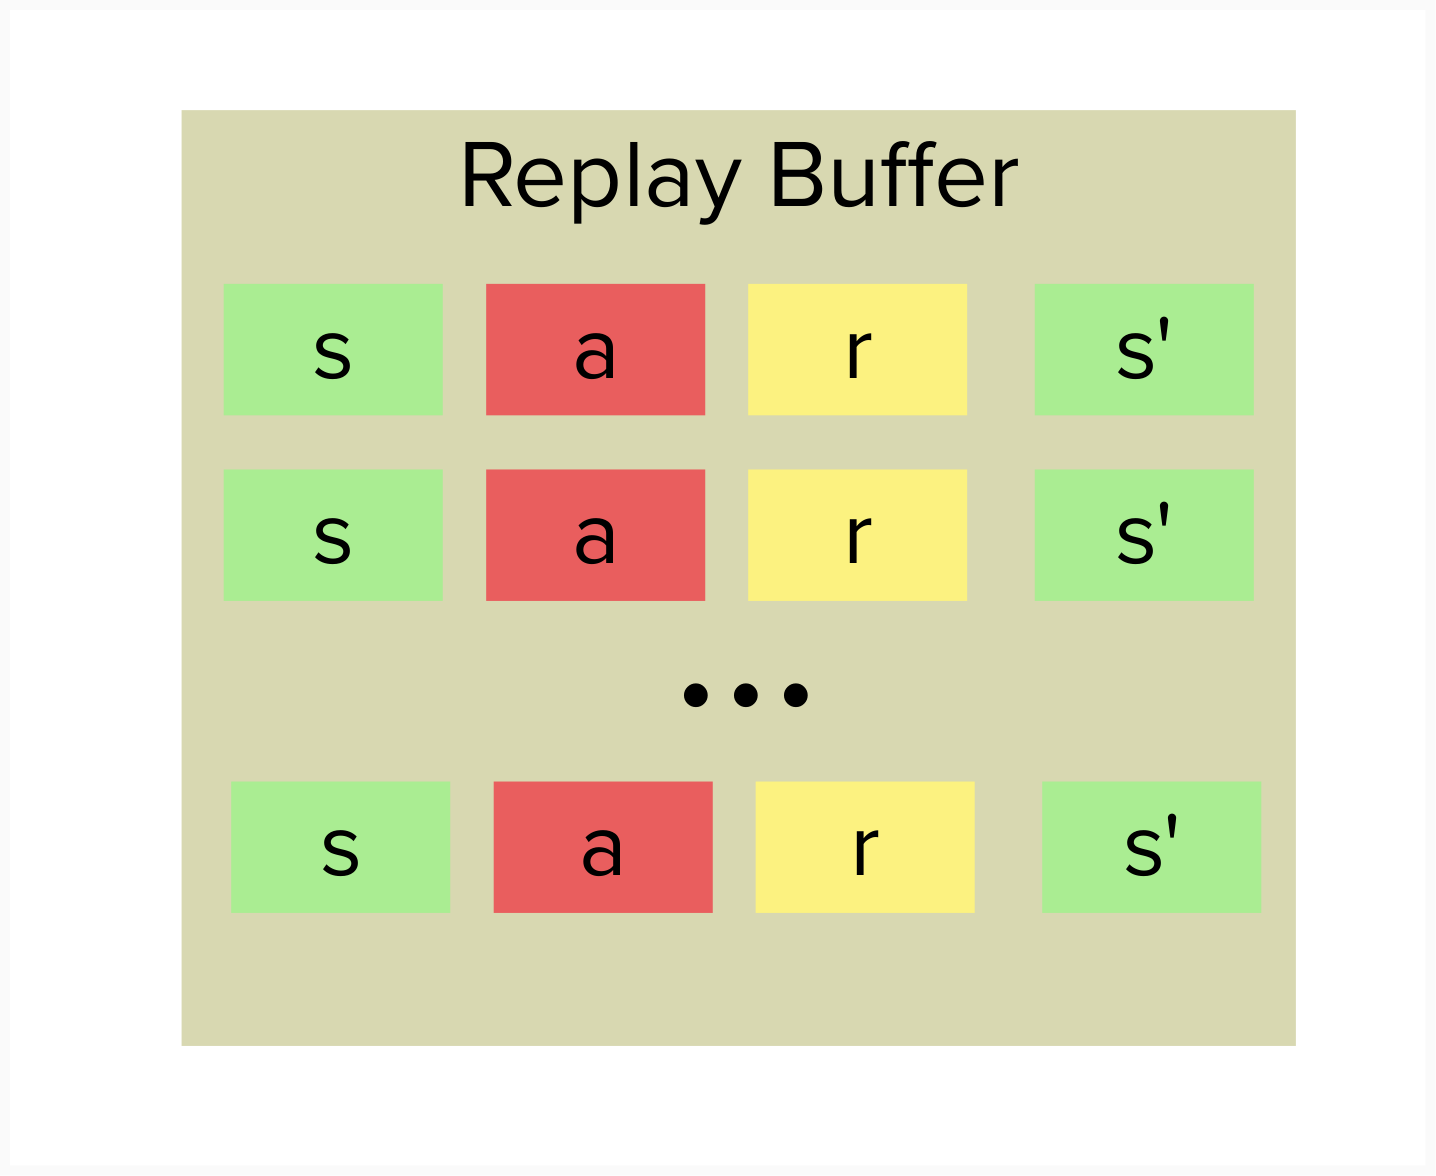
\includegraphics[width=0.5\textwidth]{3Experiment/2Experiment/1Replay_Buffer.png}
\caption{Schematische Darstellung des Replay Buffers, der die Elemente \( s \), \( a \), \( r \), und \( s' \) speichert, welche die Zustände, Aktionen, Belohnungen und Folgezustände repräsentieren.}
\label{fig:replay-buffer}
\end{figure}

Die im Replay Buffer \ref{fig:replay-buffer} gespeicherten Daten werden für das Training des neuronalen Netzes verwendet.


